\begin{definicja}[Architektura równoległa]\label{def:arch_rownolegla}
\textbf{Architektura równoległa} jest to architektura wieloprocesorowa, na której można wykonywać przetwarzanie równoległe \cite{IEEE}.
\end{definicja}

Algorytmy równoległe i architektury równoległe są ze sobą blisko spokrewnione. Równoległość może być zaimplementowana na wielu poziomach używając technik sprzętowych i programowych.
\begin{enumerate}
\item{Równoległość na poziomie danych (ang. \emph{Data-level parallelism}), gdzie pracujemy na wielu bitach danych lub na wielu danych jednocześnie.}
\item{Równoległość na poziomie instrukcji (ang. \emph{Instruction-level parallelism}, ILP), gdzie jednocześnie procesor może wykonać więcej niż jedną instrukcję.}
\item{Równoległość na poziomie wątków (ang. \emph{Thread-level parallelism}, TLP). Wątek jest częścią programu, która współdzieli zasoby procesora z innymi wątkami. W TLP wiele programowych wątków jest uruchamianych jednocześnie na jednym bądź wielu procesorach.}
\item{Równoległość na poziomie procesów (ang. \emph{Process-level parallelism}). Proces to program, który jest uruchomiany na komputerze. Rezerwuje on własne zasoby komputera, takie jak przestrzeń pamięciową i rejestry.\cite{APC2011}}
\end{enumerate}

\subsubsection{Klasyfikacja Flynna}
Architektury komputerowe można podzielić na klasy ze względu na liczbę równolegle wykonywanych instrukcji -- strumieni instrukcji oraz dostępnych strumieni danych\footnote{Strumieniem instrukcji nazywamy sekwencję instrukcji wykonywanych przez procesor, zaś strumień danych to sekwencja danych przetwarzanych przez strumień instrukcji.}. 
Klasyfikację taką (rys. \ref{fig:flynn}) zaproponował Michael J. Flynn w 1966 roku i przyjęła ona swoją nazwę od jego nazwiska (rys. \ref{fig:flynn}).

\begin{figure}
\centering
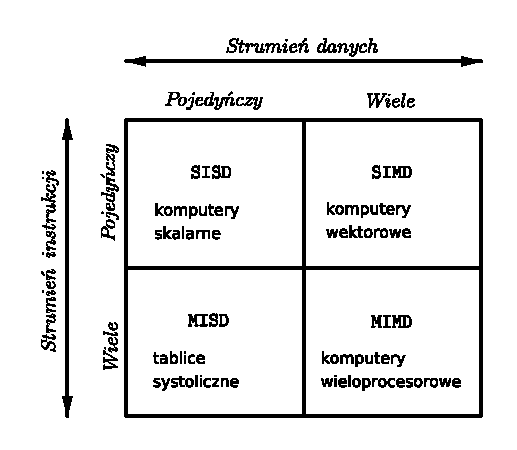
\includegraphics[width=24em]{images/flynn.eps}
\caption{Klasyfikacja Flynna}
\label{fig:flynn}
\end{figure}

\paragraph{SISD.}
Klasa SISD (ang. \emph{Single Instruction, Single Data}) odnosi się do komputerów wykonujących pojedyńczy strumień instrukcji i przetwarzających pojedyńczy strumień danych. Są to komputery całkowicie sekwencyjne, które nie wykonują żadnych obliczeń równoległych.
\paragraph{SIMD.}
Klasa SIMD (ang. \emph{Single Instruction, Multiple Data}) odnosi się do komputerów obsługujących pojedyńczy strumień instrukcji i przetwarzających wiele strumieni danych. Na różnych zbiorach danych wykownywane są te same operacje. Jako przykład takiej architektury warto wymienić przede wszystkim wczesne komputery macierzowe (nazywane niekiedy wektorowymi) ze wspólną pamięcią i macierzą jednostek przetwarzających nadzorowanych przez jednostkę sterującą, takie jak komputer ILLIAC IV wykorzystywany przez NASA w latach '70.
\paragraph{MISD.}
Klasa MISD (ang. \emph{Multiple Instruction, Single Data}) 
odnosie się do komputerów wykonujących jednocześnie wiele instrukcji przetwarzających jeden wspólny strumien danych. Przykładem takiej architektury jest tablica systoliczna\footnote{Nazwa pochodzi od skurczu mięśni serca przez analogię ,,pompowania'' danych do jednostek przetwarzających na wzór krwi w naczyniach krwionośnych.}. Tablica systoliczna jest to układ prostych jednostek przetwarzających połączonych w sieć z sąsiadującymi jednostkami, które synchronicznie wykonują pewne elementarne operacje obliczeniowe.
\paragraph{MIMD.}
Klasa MIMD  (ang. \emph{Multiple Instruction, Multiple Data})
odnosi się do komputerów równolegle wykonujących wiele instrukcji z których każda przetwarza własne strumienie danych. Do tej kategorii zaliczają się multiprocesory\footnote{Komputery z wieloma jednostkami centralnymi przyłączonymi do pamięci współdzielonej (ang. \emph{shared memory}.)} (większość współczesnych komputerów PC) i multikomputery\footnote{Wiele komputerów połączonych siecią, każdy z własną przestrzenią adresową.}. 


Większość obecnie używanych komputerów równoległych to klastry o architekturze mieszanej. Klaster jest układem niezależnych jednostek obliczeniowych (\emph{węzłów}) połączonych szybką siecią komunikacyjną. 